\chapter{THIẾT KẾ VÀ THỰC HIỆN HỆ THỐNG KIỂM THỬ TỰ ĐỘNG BẰNG ROBOT FRAMEWORK}
Trong quá trình phát triển hệ thống nhúng, đặc biệt đối với các thiết bị sử dụng nhiều giao tiếp ngoại vi hoặc các cơ chế thời gian thực, việc kiểm thử firmware đóng vai trò rất quan trọng nhằm đảm bảo hệ thống hoạt động đúng chức năng và ổn định trong nhiều điều kiện vận hành khác nhau.

Phương pháp kiểm thử thủ công truyền thống thường yêu cầu người dùng phải trực tiếp gửi lệnh, quan sát tín hiệu phản hồi, so sánh kết quả với giá trị mong đợi và ghi nhận trạng thái hoạt động của hệ thống. Quá trình này không chỉ tốn nhiều thời gian mà còn dễ phát sinh sai sót do yếu tố con người, đặc biệt khi số lượng test case lớn hoặc cần thực hiện kiểm thử lặp lại nhiều lần sau mỗi lần cập nhật firmware. Việc kiểm thử thủ công cũng gây khó khăn trong việc chuẩn hóa quy trình, đảm bảo tính nhất quán giữa các lần kiểm thử và giữa các người dùng khác nhau.

Trong hệ thống hiện tại, phần mềm giao diện được xây dựng bằng PyQt5 chủ yếu phục vụ cho việc cấu hình thiết bị, giám sát trạng thái hoạt động và hỗ trợ thao tác kiểm tra thủ công thông qua giao diện người dùng. Mặc dù phần mềm này có thể hỗ trợ thực hiện một số bài kiểm tra cơ bản, nhưng việc sử dụng giao diện đồ họa để chạy số lượng lớn test case hoặc thực hiện kiểm thử hồi quy thường xuyên vẫn còn nhiều hạn chế. Các thao tác phụ thuộc nhiều vào người vận hành, khó xây dựng quy trình kiểm thử lặp lại hoàn toàn tự động và không thuận lợi cho việc quản lý tập trung các kịch bản kiểm thử.

Đối với hệ thống Hardware-in-the-Loop, việc kiểm thử không chỉ dừng lại ở mức kiểm tra phần mềm mà còn phải đánh giá khả năng tương tác giữa DUT và các thiết bị ngoại vi được mô phỏng bởi hệ thống HIL. Các bài kiểm thử thường bao gồm nhiều bước liên tiếp như cấu hình môi trường mô phỏng, khởi tạo DUT, gửi lệnh điều khiển, thu thập dữ liệu phản hồi và đánh giá kết quả cuối cùng. Nếu thực hiện hoàn toàn thủ công hoặc phụ thuộc chủ yếu vào giao diện điều khiển bằng tay, quá trình này sẽ rất phức tạp, khó đảm bảo tính nhất quán và khó mở rộng khi số lượng bài kiểm thử tăng lên.

Bên cạnh đó, trong quá trình phát triển firmware, mỗi lần thay đổi mã nguồn đều có nguy cơ ảnh hưởng đến các chức năng đã hoạt động ổn định trước đó. Điều này đòi hỏi phải thực hiện kiểm thử hồi quy thường xuyên để phát hiện sớm các lỗi phát sinh ngoài mong muốn. Việc thực hiện kiểm thử hồi quy bằng phương pháp thủ công gần như không khả thi khi hệ thống ngày càng phức tạp, trong khi việc quản lý test case trực tiếp trong phần mềm giao diện cũng không phù hợp cho các quy trình kiểm thử quy mô lớn và lâu dài.

Vì vậy, cần xây dựng một hệ thống kiểm thử tự động độc lập với phần mềm giao diện vận hành, có khả năng tổ chức các test case theo cấu trúc rõ ràng, tự động thực hiện toàn bộ quy trình kiểm thử từ cấu hình hệ thống HIL, điều khiển DUT thực hiện các tác vụ kiểm tra, thu thập dữ liệu phản hồi cho đến đánh giá kết quả PASS/FAIL theo các tiêu chí đã định trước. Hệ thống này giúp giảm đáng kể thời gian kiểm thử, tăng độ chính xác, nâng cao khả năng lặp lại của các bài test và hỗ trợ phát hiện lỗi sớm trong quá trình phát triển sản phẩm.

\section{Lựa chọn Robot Framework cho hệ thống kiểm thử tự động}

Để xây dựng hệ thống kiểm thử tự động cho mô hình Hardware-in-the-Loop, có nhiều phương pháp có thể được lựa chọn như sử dụng Python thuần, unittest, pytest hoặc các công cụ kiểm thử tự động chuyên dụng khác. Mỗi phương pháp đều có những ưu điểm và hạn chế riêng tùy thuộc vào đặc điểm hệ thống cần kiểm thử.

Sử dụng Python thuần cho phép lập trình viên toàn quyền kiểm soát luồng xử lý, dễ dàng xây dựng các hàm giao tiếp phần cứng phức tạp và tối ưu theo từng yêu cầu cụ thể. Tuy nhiên, khi số lượng test case tăng lên, việc quản lý các kịch bản kiểm thử hoàn toàn bằng mã nguồn trở nên khó kiểm soát, khó bảo trì và phụ thuộc nhiều vào kỹ năng lập trình của người viết test. Ngoài ra, việc chuẩn hóa cấu trúc test case, tổ chức báo cáo kết quả và thực hiện kiểm thử hồi quy cũng đòi hỏi phải tự xây dựng thêm nhiều thành phần hỗ trợ.

Các framework như unittest hoặc pytest phù hợp với kiểm thử phần mềm thông thường, đặc biệt là unit test hoặc integration test ở mức hàm và module. Tuy nhiên, đối với hệ thống nhúng có sự tham gia của DUT, HIL và nhiều giao tiếp ngoại vi như UART, I2C, SPI, CAN, việc mô tả các bước kiểm thử theo hướng thao tác thiết bị thực tế sẽ trở nên khó trực quan nếu chỉ sử dụng các framework này. Các test case thường bị gắn chặt với mã nguồn Python, gây khó khăn cho việc theo dõi, bảo trì và mở rộng lâu dài.

Với yêu cầu cần một hệ thống kiểm thử có cấu trúc rõ ràng, dễ quản lý và thuận tiện cho kiểm thử hồi quy, một nền tảng hỗ trợ tổ chức test case theo hướng trực quan và tách biệt với phần xử lý phần cứng là cần thiết. Robot Framework đáp ứng tốt yêu cầu này nhờ hoạt động theo mô hình keyword-driven testing.

Robot Framework là một nền tảng kiểm thử tự động mã nguồn mở hoạt động theo mô hình keyword-driven testing. Trong mô hình này, dữ liệu kiểm thử (Test Data) được xây dựng dưới dạng các test case và keyword mô tả từng bước kiểm tra. Robot Framework đóng vai trò trung tâm điều phối, tiếp nhận các test case này và gọi các thư viện kiểm thử (Test Library) để thực hiện các thao tác thực tế trên hệ thống cần kiểm thử (System Under Test).

Các thư viện kiểm thử có thể là các thư viện có sẵn của Robot Framework hoặc các thư viện Python tự phát triển nhằm phục vụ các yêu cầu đặc thù của hệ thống nhúng như gửi lệnh UART, đọc phản hồi từ DUT, cấu hình môi trường mô phỏng HIL hoặc kiểm tra tín hiệu ngoại vi. Nhờ kiến trúc phân lớp này, phần mô tả test case được tách biệt rõ ràng khỏi phần xử lý giao tiếp phần cứng, giúp hệ thống dễ bảo trì và dễ mở rộng hơn.

\begin{figure}[H]
    \centering
    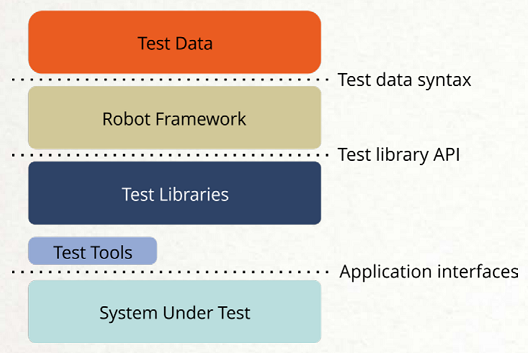
\includegraphics[width=0.85\textwidth]{image/robot_framework_structure.png}
    \caption{Cấu trúc hoạt động của Robot Framework}
    \label{fig:robot_framework_structure}
\end{figure}

Trong phương pháp keyword-driven testing, mỗi thao tác kiểm thử được xây dựng dưới dạng các keyword có ý nghĩa rõ ràng như gửi lệnh, đọc phản hồi, kiểm tra dữ liệu hoặc xác nhận trạng thái hệ thống. Nhờ đó, các test case được biểu diễn dưới dạng các bước kiểm thử trực quan, dễ đọc và gần với quy trình kiểm thử thực tế hơn so với việc viết hoàn toàn bằng mã nguồn Python.

Ưu điểm lớn nhất của Robot Framework là khả năng chuẩn hóa cấu trúc test case và tách biệt rõ ràng giữa phần logic kiểm thử với phần xử lý giao tiếp phần cứng. Các thao tác phức tạp như gửi lệnh UART, cấu hình EEPROM giả lập, điều khiển RTC, đọc dữ liệu Logic Analyzer hoặc kiểm tra tín hiệu PWM có thể được xây dựng trong các thư viện Python tự phát triển, sau đó đóng gói thành các keyword đơn giản để tái sử dụng trong nhiều test case khác nhau. Điều này giúp hệ thống vừa giữ được tính linh hoạt của Python, vừa đảm bảo khả năng quản lý tập trung và dễ bảo trì.

Bên cạnh đó, Robot Framework hỗ trợ tự động sinh báo cáo kiểm thử dưới dạng log, report và thống kê kết quả PASS/FAIL sau mỗi lần thực thi. Đây là một ưu điểm rất quan trọng trong kiểm thử firmware vì giúp kỹ sư dễ dàng theo dõi kết quả, phân tích lỗi và thực hiện kiểm thử hồi quy sau mỗi lần cập nhật firmware mà không cần xây dựng thêm hệ thống báo cáo riêng.

Tuy nhiên, Robot Framework cũng tồn tại một số hạn chế. Đối với các bài kiểm thử có logic xử lý quá phức tạp hoặc yêu cầu kiểm soát rất chi tiết ở mức thấp, việc biểu diễn hoàn toàn bằng keyword có thể trở nên cồng kềnh hơn so với viết trực tiếp bằng Python. Ngoài ra, hiệu năng thực thi của Robot Framework thường không tối ưu bằng chương trình Python thuần trong các tác vụ yêu cầu xử lý tốc độ rất cao. Vì vậy, Robot Framework phù hợp nhất khi được sử dụng như một lớp điều phối kiểm thử, trong khi các thao tác phần cứng phức tạp vẫn được xử lý bởi các thư viện Python chuyên biệt.

Trong phạm vi đề tài này, mục tiêu chính là xây dựng một hệ thống kiểm thử tự động có khả năng tổ chức test case rõ ràng, dễ mở rộng, dễ bảo trì và hỗ trợ kiểm thử hồi quy lâu dài cho hệ thống HIL. Do đó, Robot Framework là lựa chọn phù hợp hơn so với Python thuần hoặc các framework kiểm thử thông thường. Việc kết hợp Robot Framework với các thư viện Python tự phát triển giúp tận dụng được ưu điểm của cả hai phương pháp, vừa đảm bảo khả năng kiểm soát giao tiếp phần cứng, vừa xây dựng được một hệ thống kiểm thử chuyên nghiệp, có khả năng mở rộng trong tương lai.

\section{Yêu cầu thiết kế}

Hệ thống kiểm thử tự động được xây dựng nhằm hỗ trợ kiểm thử firmware của DUT trong môi trường Hardware-in-the-Loop một cách chính xác, ổn định và có khả năng mở rộng. Để đáp ứng yêu cầu này, hệ thống cần thỏa mãn các tiêu chí thiết kế sau:

\begin{itemize}

    \item Hệ thống phải cung cấp một thư viện các hàm kiểm thử chuyên biệt để giao tiếp với DUT và HIL, bao gồm các thao tác như gửi lệnh điều khiển, đọc dữ liệu phản hồi, cấu hình môi trường mô phỏng và đánh giá kết quả kiểm thử.

    \item Kiến trúc hệ thống phải đảm bảo tính mở rộng và khả năng bảo trì lâu dài, cho phép dễ dàng bổ sung thư viện mới, xây dựng thêm các kịch bản kiểm thử và cập nhật khi có thay đổi về phần cứng hoặc yêu cầu kiểm thử mới trong quá trình phát triển firmware.

    \item Các kịch bản kiểm thử phải được tổ chức theo cấu trúc rõ ràng, dễ đọc, dễ hiểu và có khả năng tái sử dụng cao, giúp thuận tiện cho việc quản lý, kiểm tra và mở rộng hệ thống kiểm thử trong tương lai.

    \item Hệ thống cần hỗ trợ giao tiếp đồng thời với DUT và hệ thống HIL thông qua các giao tiếp như USB hoặc UART, đảm bảo khả năng điều khiển thiết bị và thu thập dữ liệu phản hồi theo thời gian thực.

    \item Hệ thống phải hỗ trợ cơ chế đánh giá kết quả kiểm thử tự động theo tiêu chí PASS/FAIL dựa trên các giá trị mong đợi đã được định nghĩa trước, hạn chế tối đa sự can thiệp thủ công của người vận hành.

    \item Toàn bộ dữ liệu kiểm thử bao gồm lệnh điều khiển, phản hồi từ DUT, trạng thái của HIL và kết quả đánh giá cần được ghi nhận đầy đủ nhằm phục vụ việc phân tích lỗi, debug firmware và truy vết kết quả kiểm thử.

    \item Hệ thống phải hỗ trợ thực hiện kiểm thử đồng thời nhiều test case, cho phép chạy các kịch bản kiểm thử liên tiếp hoặc song song để tối ưu hóa thời gian kiểm thử, đặc biệt trong các tình huống cần thực hiện kiểm thử hồi quy sau mỗi lần cập nhật firmware.

\end{itemize}

Cấu trúc triển khai cụ thể của hệ thống kiểm thử tự động trong môi trường Hardware-in-the-Loop được trình bày trong Hình \ref{fig:hil_robot_structure}.

\begin{figure}[H]
    \centering
    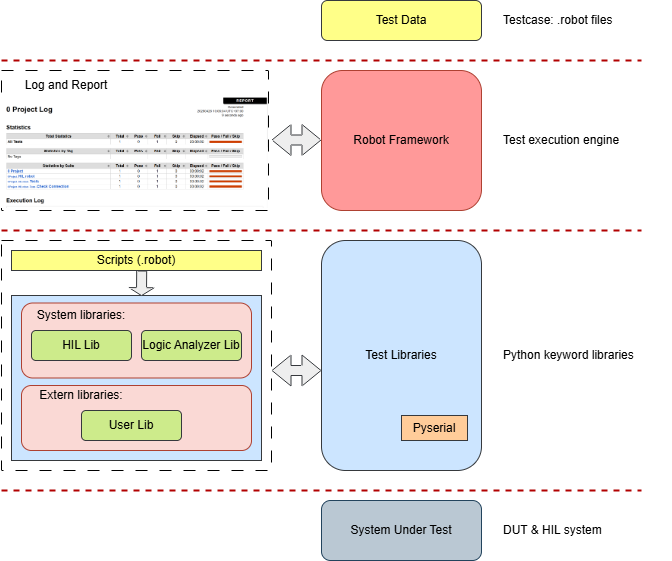
\includegraphics[width=0.85\textwidth]{image/hil_robot_structure.png}
    \caption{Cấu trúc triển khai Robot Framework trong hệ thống HIL}
    \label{fig:hil_robot_structure}
\end{figure}

Khác với cấu trúc tổng quan của Robot Framework đã trình bày ở phần trước, hình \ref{fig:hil_robot_structure} mô tả cách hệ thống kiểm thử được triển khai cụ thể trong phạm vi đề tài.

Các test case được xây dựng dưới dạng các file \texttt{.robot}, trong đó mỗi bài kiểm thử tương ứng với một chức năng ngoại vi như GPIO, PWM, UART, I2C, SPI hoặc CAN. Mỗi test case bao gồm các bước cấu hình môi trường kiểm thử, điều khiển DUT thực hiện tác vụ cần kiểm tra, thu thập dữ liệu phản hồi và đánh giá kết quả cuối cùng.

Robot Framework đóng vai trò điều phối trung tâm, thực thi tuần tự các test case và gọi các keyword tương ứng trong các thư viện kiểm thử. Đối với hệ thống HIL và Logic Analyzer, các keyword được xây dựng sẵn và lưu trữ trong thư viện hệ thống. Các keyword này tương ứng trực tiếp với toàn bộ tập lệnh được hỗ trợ bởi HIL và Logic Analyzer, cho phép thực hiện các thao tác gửi lệnh, nhận phản hồi và cấu hình môi trường mô phỏng. Bên cạnh đó, hệ thống cũng cung cấp thêm các keyword tiện ích phục vụ kiểm thử như kiểm tra trạng thái thiết bị, so sánh giá trị phản hồi với giá trị mong đợi và xác nhận kết quả PASS/FAIL.

Đối với DUT, thư viện kiểm thử được xây dựng riêng tùy theo từng thiết bị cần kiểm tra, dựa trên tập lệnh và yêu cầu chức năng cụ thể của firmware và sẽ do người dùng xây dựng. Cách tổ chức này giúp hệ thống có tính linh hoạt cao, dễ dàng mở rộng cho nhiều loại DUT khác nhau mà không ảnh hưởng đến kiến trúc tổng thể của hệ thống kiểm thử.

Tầng giao tiếp vật lý sử dụng thư viện \texttt{pyserial} để kết nối với DUT, HIL và Logic Analyzer thông qua cổng USB serial. Thư viện này chịu trách nhiệm thực hiện truyền nhận dữ liệu, đồng bộ quá trình kiểm thử và đảm bảo luồng giao tiếp ổn định giữa các thiết bị trong suốt quá trình thực thi test case.

Sau khi quá trình kiểm thử hoàn tất, Robot Framework tự động sinh ra các tệp báo cáo như \texttt{report.html}, \texttt{log.html} và \texttt{output.xml}. Trong đó, \texttt{report.html} cung cấp kết quả tổng quan của toàn bộ quá trình kiểm thử với trạng thái PASS/FAIL của từng test case, \texttt{log.html} ghi lại chi tiết từng bước thực thi, các lệnh đã gửi, dữ liệu phản hồi và thông tin debug trong quá trình kiểm thử, còn \texttt{output.xml} được sử dụng để lưu trữ dữ liệu kết quả dưới dạng có cấu trúc phục vụ cho việc phân tích hoặc tích hợp với các hệ thống kiểm thử khác. Việc tự động ghi nhận log và sinh báo cáo giúp kỹ sư dễ dàng truy vết lỗi, đánh giá chất lượng firmware và thực hiện kiểm thử hồi quy một cách hiệu quả.

Nhờ cấu trúc phân lớp này, hệ thống kiểm thử vừa đảm bảo tính tự động hóa cao, vừa dễ dàng mở rộng khi cần bổ sung thêm ngoại vi mới hoặc xây dựng thêm các bài kiểm thử trong tương lai.


\section{Thiết kế các kịch bản kiểm thử}

Dựa trên kiến trúc hệ thống kiểm thử đã xây dựng cùng tập các keyword hỗ trợ cho HIL và Logic Analyzer, bước tiếp theo là thiết kế các kịch bản kiểm thử cụ thể cho từng chức năng ngoại vi của DUT. Các keyword được sử dụng như những khối chức năng cơ bản để xây dựng quy trình kiểm thử hoàn chỉnh, bao gồm thiết lập môi trường kiểm thử, điều khiển DUT và HIL, thu thập dữ liệu phản hồi cũng như đánh giá kết quả theo tiêu chí PASS/FAIL.

Mỗi kịch bản kiểm thử được xây dựng nhằm xác minh tính đúng đắn của firmware khi thực hiện giao tiếp với các thiết bị ngoại vi được mô phỏng bởi hệ thống HIL.

Phần tiếp theo trình bày lưu đồ giải thuật chi tiết của một số nhóm test case tiêu biểu được triển khai trong đề tài.

\subsection{Kiểm tra kết nối của HIL và DUT}

Mục đích của bài kiểm thử này là xác minh khả năng kết nối và giao tiếp giữa PC với HIL, đồng thời giữa PC với DUT, nhằm đảm bảo toàn bộ hệ thống sẵn sàng cho các bài kiểm thử chức năng tiếp theo.

Quy trình kiểm thử bao gồm các bước sau:

\begin{itemize}
    \item Bước 1: Kết nối HIL với PC thông qua cổng USB serial và kiểm tra khả năng nhận diện thiết bị.
    \item Bước 2: Cấp nguồn cho DUT thông qua hệ thống HIL để chuẩn bị cho quá trình kiểm thử.
    \item Bước 3: Kết nối DUT với PC thông qua cổng USB hoặc UART và xác nhận thiết bị có thể giao tiếp.
    \item Bước 4: Gửi lệnh kiểm tra cơ bản từ PC đến HIL và DUT, thu thập phản hồi để xác minh khả năng giao tiếp hai chiều.
    \item Bước 5: Đánh giá kết quả kiểm thử dựa trên phản hồi nhận được.
\end{itemize}

Điều kiện đánh giá:

\begin{itemize}
    \item PASS: HIL và DUT đều được nhận diện đúng, có thể giao tiếp và phản hồi chính xác lệnh kiểm tra.
    \item FAIL: Ít nhất một trong hai thiết bị không được nhận diện, không thể giao tiếp hoặc phản hồi không chính xác.
\end{itemize}

Lưu đồ giải thuật tổng quát của bài kiểm thử được trình bày trong Hình \ref{fig:connection_test_flowchart}.

\begin{figure}[H]
    \centering
    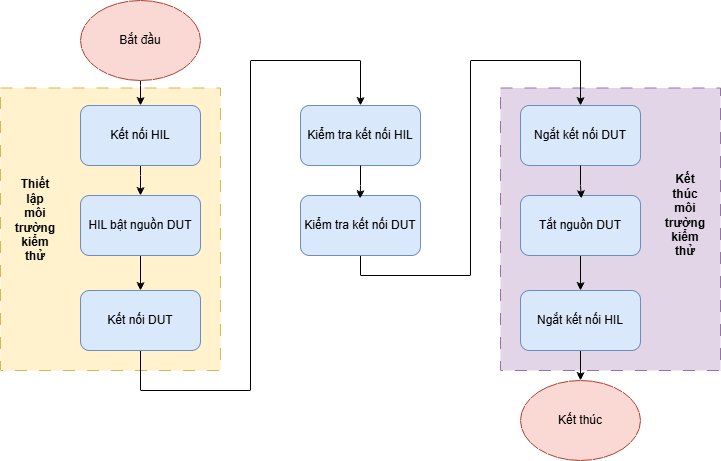
\includegraphics[width=0.8\textwidth]{image/connection_test_flowchart.png}
    \caption{Lưu đồ giải thuật kiểm tra kết nối HIL và DUT}
    \label{fig:connection_test_flowchart}
\end{figure}

Đây là bài kiểm thử cơ bản nhất nhằm đảm bảo hệ thống đã được thiết lập đúng trước khi thực hiện các bài kiểm thử chức năng khác. Trong đó, ba bước đầu gồm kết nối HIL, cấp nguồn cho DUT và kết nối DUT sẽ được quy ước là giai đoạn thiết lập môi trường kiểm thử. Tương tự, các bước ngắt kết nối DUT, tắt nguồn DUT và ngắt kết nối HIL ở cuối quá trình được quy ước là giai đoạn kết thúc môi trường kiểm thử.

Giữa hai giai đoạn này là phần kiểm thử chính, được thay đổi tùy theo yêu cầu của từng test case cụ thể. Đối với bài kiểm tra kết nối, thao tác chính là gửi lệnh kiểm tra cơ bản như \texttt{help} đến HIL và DUT, sau đó thu thập phản hồi và so sánh với giá trị mong đợi để xác minh trạng thái hoạt động của thiết bị.

Lưu đồ giải thuật chi tiết cho quá trình xác minh kết nối được trình bày trong Hình \ref{fig:verify_connection_flowchart}.

\begin{figure}[H]
    \centering
    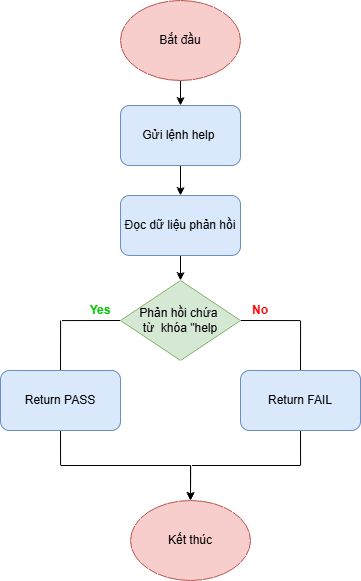
\includegraphics[height=0.4\textheight]{image/verify_connection_flowchart.png}
    \caption{Lưu đồ giải thuật xác minh kết nối của HIL và DUT với PC}
    \label{fig:verify_connection_flowchart}
\end{figure}

\subsection{Kiểm tra khả năng flash firmware cho DUT}

Mục đích của bài kiểm thử này là xác minh khả năng nạp firmware mới cho DUT thông qua hệ thống HIL, đảm bảo quá trình cập nhật chương trình được thực hiện đúng, ổn định và DUT có thể khởi động lại với firmware mới sau khi hoàn tất.

Quy trình kiểm thử bao gồm các bước sau:

\begin{itemize}
    \item Bước 1: Kiểm tra kết nối giữa PC, HIL và DUT, đảm bảo hệ thống sẵn sàng cho quá trình nạp firmware.
    \item Bước 2: Tắt nguồn DUT và điều khiển chân BOOT0 ở mức cao thông qua HIL để đưa DUT vào chế độ DFU (Device Firmware Upgrade).
    \item Bước 3: Cấp nguồn lại cho DUT và kiểm tra việc nhận diện thiết bị DFU trên máy tính.
    \item Bước 4: Sử dụng công cụ STM32CubeProgrammer CLI để thực hiện nạp firmware vào bộ nhớ Flash của DUT.
    \item Bước 5: Sau khi nạp hoàn tất, đưa chân BOOT0 về mức thấp và khởi động lại DUT để chạy chương trình mới.
    \item Bước 6: Kiểm tra phản hồi từ DUT nhằm xác minh firmware đã được nạp thành công và hệ thống hoạt động bình thường.
\end{itemize}

Điều kiện đánh giá:

\begin{itemize}
    \item PASS: DUT được nhận diện đúng ở chế độ DFU, firmware được nạp thành công, xác minh Flash hợp lệ và DUT khởi động lại bình thường với chương trình mới.
    \item FAIL: Bài kiểm thử sẽ trả về FAILD nếu gặp bất kì lỗi nào sau đây: DUT không vào được chế độ DFU, quá trình nạp firmware thất bại, xác minh Flash lỗi hoặc DUT không hoạt động đúng sau khi khởi động lại.
\end{itemize}

Lưu đồ giải thuật tổng quát của bài kiểm thử được trình bày trong Hình \ref{fig:flash_fw_flowchart}.

\begin{figure}[H]
    \centering
    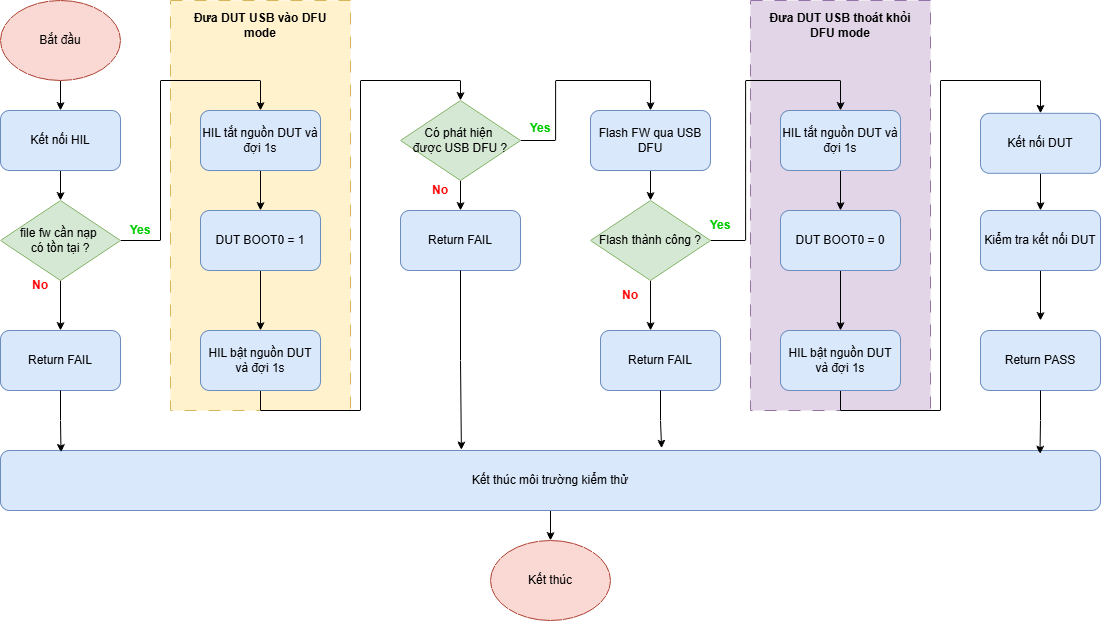
\includegraphics[width=0.8\textwidth]{image/flash_fw_flowchart.png}
    \caption{Lưu đồ giải thuật kiểm tra khả năng flash firmware cho DUT}
    \label{fig:flash_fw_flowchart}
\end{figure}

Trong bài kiểm thử này, hệ thống HIL đóng vai trò hỗ trợ điều khiển phần cứng của DUT, bao gồm bật/tắt nguồn và điều khiển chân BOOT0 để chuyển DUT vào chế độ bootloader. Sau đó, Robot Framework sử dụng thư viện Python để gọi công cụ STM32CubeProgrammer CLI thực hiện quá trình nạp firmware tự động.

Sau khi hoàn tất quá trình ghi Flash, DUT được đưa trở lại chế độ hoạt động bình thường bằng cách đưa BOOT0 về mức thấp và thực hiện reset nguồn. Bước cuối cùng là xác minh DUT có thể khởi động thành công với firmware mới, đảm bảo toàn bộ quá trình cập nhật chương trình diễn ra chính xác và ổn định.

\subsection{Kiểm tra ngoại vi GPIO}
Mục đích của bài kiểm thử này là xác minh khả năng điều khiển và phản hồi tín hiệu GPIO của DUT ở cả hai chế độ GPIO Output và GPIO Input. Bài kiểm thử nhằm đảm bảo firmware cấu hình đúng chế độ hoạt động của chân GPIO, đồng thời tín hiệu thực tế tại chân vi điều khiển phù hợp với trạng thái mong đợi trong từng trường hợp kiểm thử.

Đối với GPIO Output, DUT chủ động xuất mức logic ra các chân điều khiển LED và hệ thống HIL thực hiện giám sát trạng thái tín hiệu thực tế tại các chân này. Đối với GPIO Input, HIL đóng vai trò tạo tín hiệu mức logic đầu vào, trong khi DUT thực hiện đọc trạng thái chân GPIO và phản hồi kết quả về PC để xác minh tính đúng đắn của quá trình nhận tín hiệu.

Quy trình kiểm thử tổng quát bao gồm các bước sau:

\begin{itemize}
    \item Bước 1: Thiết lập môi trường kiểm thử bằng cách kết nối HIL, cấp nguồn cho DUT và thiết lập kết nối với DUT.
    \item Bước 2: Thực hiện bài kiểm thử GPIO Output, trong đó DUT điều khiển trạng thái các chân GPIO đầu ra và HIL kiểm tra mức logic thực tế tại các chân tương ứng.
    \item Bước 3: Thực hiện bài kiểm thử GPIO Input, trong đó HIL tạo tín hiệu mức logic đầu vào và DUT đọc trạng thái các chân GPIO để xác minh kết quả nhận được.
    \item Bước 4: Đánh giá kết quả kiểm thử dựa trên toàn bộ phản hồi thu được từ cả hai bài kiểm thử.
    \item Bước 5: Kết thúc môi trường kiểm thử bằng cách ngắt kết nối DUT, tắt nguồn DUT và ngắt kết nối HIL.
\end{itemize}

Điều kiện đánh giá:

\begin{itemize}
    \item PASS: Tất cả các chân GPIO ở cả hai chế độ Output và Input đều hoạt động đúng, tín hiệu đọc được từ HIL và DUT khớp với giá trị mong đợi.
    \item FAIL: Có ít nhất một chân GPIO không thay đổi đúng trạng thái hoặc giá trị đọc được không khớp với trạng thái mong đợi.
\end{itemize}

Lưu đồ giải thuật tổng quát của bài kiểm thử được trình bày trong Hình \ref{fig:gpio_test_flowchart}.

\begin{figure}[H]
    \centering
    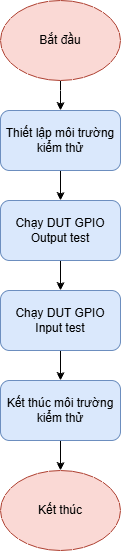
\includegraphics[height=0.4\textheight]{image/gpio_test_flowchart.png}
    \caption{Lưu đồ giải thuật tổng quát kiểm tra chức năng GPIO}
    \label{fig:gpio_test_flowchart}
\end{figure}

Trong bài kiểm thử GPIO Output, DUT đóng vai trò chủ động điều khiển trạng thái logic các chân GPIO. Hệ thống HIL sẽ đọc trực tiếp mức logic tại các chân này và so sánh với giá trị mong đợi để xác minh tính chính xác của tín hiệu đầu ra.

Lưu đồ giải thuật chi tiết của phần kiểm thử GPIO Output được trình bày trong Hình \ref{fig:gpio_output_test_flowchart}.

\begin{figure}[H]
    \centering
    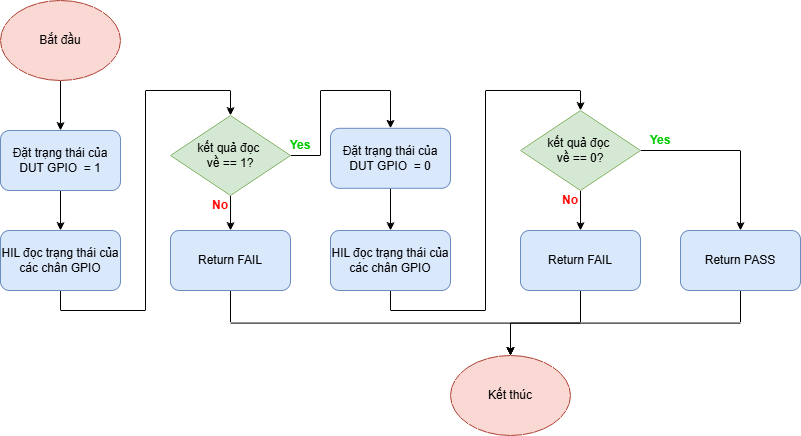
\includegraphics[width=0.8\textwidth]{image/gpio_output_test_flowchart.png}
    \caption{Lưu đồ giải thuật kiểm tra GPIO Output}
    \label{fig:gpio_output_test_flowchart}
\end{figure}

Trong bài kiểm thử GPIO Input, vai trò giữa DUT và HIL được thực hiện theo hướng ngược lại. HIL đóng vai trò chủ động điều khiển trạng thái logic các chân GPIO. DUT sẽ đọc trực tiếp mức logic tại các chân này và so sánh với giá trị mong đợi để xác minh tính chính xác của tín hiệu đầu ra.

Lưu đồ giải thuật chi tiết của phần kiểm thử GPIO Input được trình bày trong Hình \ref{fig:gpio_input_test_flowchart}.

\begin{figure}[H]
    \centering
    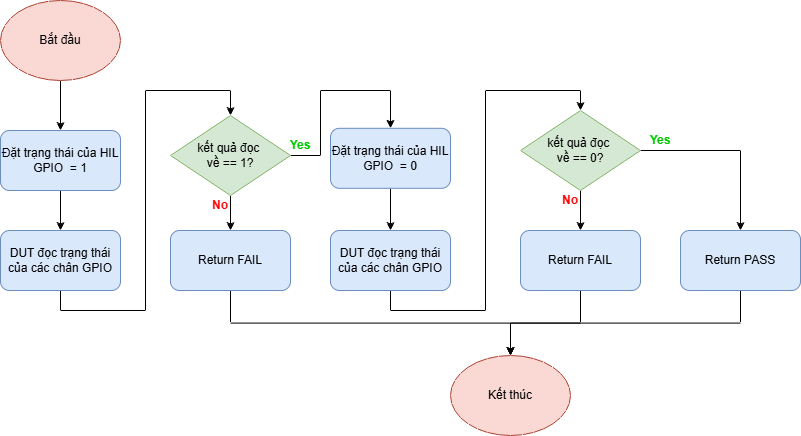
\includegraphics[width=0.8\textwidth]{image/gpio_input_test_flowchart.png}
    \caption{Lưu đồ giải thuật kiểm tra GPIO Input}
    \label{fig:gpio_input_test_flowchart}
\end{figure}

\subsection{Kiểm tra ngoại vi ADC}

Mục đích của bài kiểm thử này là xác minh khả năng đọc tín hiệu analog của DUT thông qua bộ chuyển đổi tương tự sang số. Bài kiểm thử nhằm đảm bảo firmware cần kiểm thử cấu hình đúng chức năng ADC, đồng thời giá trị điện áp đo được từ DUT phản ánh chính xác tín hiệu đầu vào do hệ thống HIL cung cấp.

Trong bài kiểm thử này, hệ thống HIL đóng vai trò tạo tín hiệu điện áp analog đầu vào thông qua ngõ ra DAC với các mức điện áp xác định trước. DUT thực hiện đọc giá trị điện áp tại chân ADC, sau đó phản hồi kết quả đo về PC để tiến hành so sánh với giá trị mong đợi.

Quy trình kiểm thử tổng quát bao gồm các bước sau:

\begin{itemize}
    \item Bước 1: Thiết lập môi trường kiểm thử bằng cách kết nối HIL, cấp nguồn cho DUT và thiết lập kết nối với DUT.
    \item Bước 2: Hệ thống HIL lần lượt thiết lập các mức điện áp đầu ra DAC tương ứng với các giá trị kiểm thử: 1.5V, 2.0V, 3.0V và 3.3V.
    \item Bước 3: Sau mỗi lần thiết lập điện áp, DUT thực hiện đọc giá trị ADC tại chân đầu vào tương ứng.
    \item Bước 4: DUT gửi kết quả đo được về PC, hệ thống tiến hành so sánh với giá trị điện áp mong đợi trong khoảng sai số cho phép.
    \item Bước 5: Đánh giá kết quả kiểm thử dựa trên toàn bộ phản hồi thu được.
    \item Bước 6: Kết thúc môi trường kiểm thử bằng cách ngắt kết nối DUT, tắt nguồn DUT và ngắt kết nối HIL.
\end{itemize}

Điều kiện đánh giá:

\begin{itemize}
    \item PASS: Tất cả các giá trị điện áp đo được từ DUT nằm trong khoảng sai số cho phép so với giá trị điện áp đầu vào do HIL cung cấp.
    \item FAIL: Có ít nhất một giá trị đo không nằm trong khoảng sai số cho phép hoặc DUT không phản hồi kết quả đo.
\end{itemize}

Lưu đồ giải thuật tổng quát của bài kiểm thử được trình bày trong Hình \ref{fig:adc_test_flowchart}.

\begin{figure}[H]
    \centering
    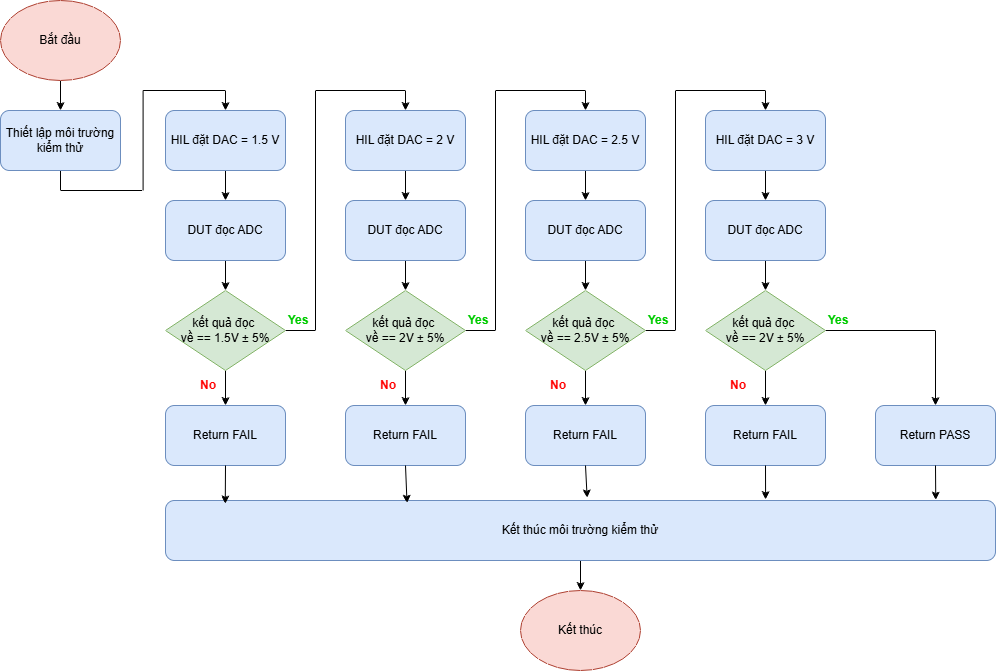
\includegraphics[width=0.7\textwidth]{image/adc_test_flowchart.png}
    \caption{Lưu đồ giải thuật kiểm tra chức năng ADC}
    \label{fig:adc_test_flowchart}
\end{figure}

Trong bài kiểm thử này, hệ thống HIL sử dụng DAC để tạo ra các mức điện áp chuẩn làm tín hiệu đầu vào cho DUT. Việc lựa chọn nhiều mức điện áp khác nhau giúp đánh giá khả năng hoạt động của ADC trên nhiều vùng đo, từ mức điện áp thấp đến mức điện áp gần ngưỡng cực đại của hệ thống.

Firmware trên DUT thực hiện đọc giá trị ADC và chuyển đổi kết quả đo thành giá trị điện áp tương ứng. Giá trị này được gửi về PC thông qua giao tiếp serial để phục vụ quá trình đánh giá.

Hệ thống kiểm thử sẽ so sánh giá trị điện áp DUT đo được với giá trị điện áp do HIL thiết lập trong một khoảng sai số cho phép ( $\pm 5\%$). Việc sử dụng khoảng sai số này giúp phản ánh đúng đặc tính thực tế của bộ ADC, bao gồm sai số chuyển đổi, sai số điện áp tham chiếu và nhiễu tín hiệu trong quá trình đo.

\subsection{Kiểm tra ngoại vi DAC}

Mục đích của bài kiểm thử này là xác minh khả năng tạo tín hiệu analog của DUT thông qua bộ chuyển đổi số sang tương tự (DAC). Bài kiểm thử nhằm đảm bảo firmware cấu hình đúng chức năng DAC, đồng thời tín hiệu analog đầu ra thực tế của DUT đáp ứng đúng dạng sóng và tần số theo yêu cầu thiết kế.

Trong bài kiểm thử này, DUT đóng vai trò chủ động phát sinh tín hiệu analog dưới dạng sóng sine và sóng tam giác với tần số xác định trước. Hệ thống Logic Analyzer được sử dụng để thu thập trực tiếp tín hiệu analog tại chân DAC, sau đó dữ liệu được xử lý và phân tích bằng thuật toán FFT nhằm xác minh đặc tính của dạng sóng đầu ra.

Quy trình kiểm thử tổng quát bao gồm các bước sau:

\begin{itemize}
    \item Bước 1: Thiết lập môi trường kiểm thử bằng cách kết nối HIL, Logic Analyzer, cấp nguồn cho DUT và thiết lập kết nối với DUT.
    \item Bước 2: DUT thực hiện phát tín hiệu sóng sine với tần số xác định trước.
    \item Bước 3: Logic Analyzer thu thập dữ liệu tín hiệu analog tại chân DAC và hệ thống thực hiện phân tích để xác minh tín hiệu có đúng dạng sóng sine và đúng tần số mong đợi hay không.
    \item Bước 4: DUT tiếp tục phát tín hiệu sóng tam giác với tần số xác định trước.
    \item Bước 5: Logic Analyzer tiếp tục thu thập dữ liệu và hệ thống thực hiện phân tích để xác minh tín hiệu có đúng dạng sóng tam giác và đúng tần số mong đợi hay không.
    \item Bước 6: Kết thúc môi trường kiểm thử bằng cách ngắt kết nối DUT, tắt nguồn DUT, ngắt kết nối Logic Analyzer và HIL.
\end{itemize}

Điều kiện đánh giá:

\begin{itemize}
    \item PASS: DUT phát đúng dạng sóng sine và sóng tam giác theo yêu cầu, tần số đo được nằm trong sai số cho phép và các đặc trưng phổ tần phù hợp với dạng sóng mong đợi.
    \item FAIL: Dạng sóng đầu ra không đúng yêu cầu, tần số sai lệch vượt giới hạn cho phép hoặc dữ liệu thu thập không đủ để thực hiện phân tích.
\end{itemize}

Lưu đồ giải thuật tổng quát của bài kiểm thử được trình bày trong Hình \ref{fig:dac_test_flowchart}.

\begin{figure}[H]
    \centering
    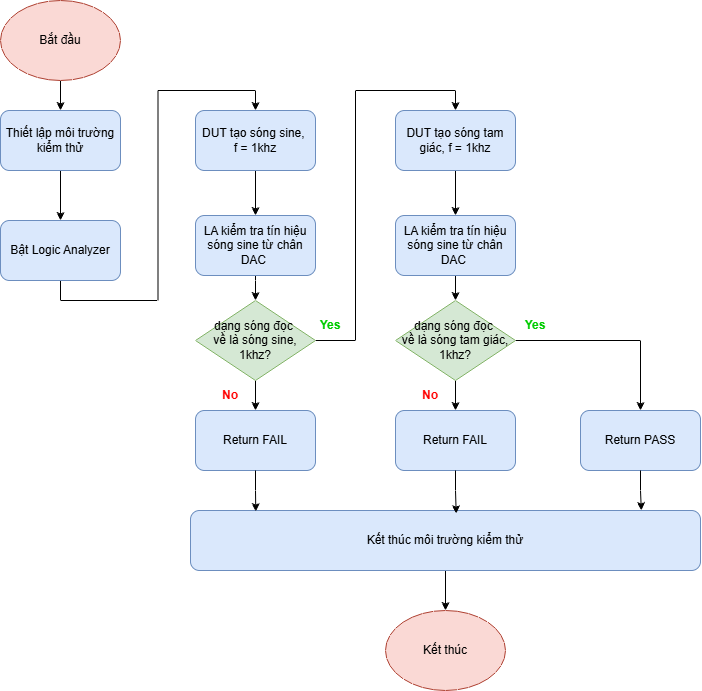
\includegraphics[width=0.8\textwidth]{image/dac_test_flowchart.png}
    \caption{Lưu đồ giải thuật tổng quát kiểm tra chức năng DAC}
    \label{fig:dac_test_flowchart}
\end{figure}

Đối với bài kiểm tra sóng sine, dữ liệu analog thu được từ Logic Analyzer sẽ được chuyển đổi sang miền tần số bằng thuật toán FFT. Hệ thống tiến hành xác định đỉnh năng lượng chính và tính tỷ lệ năng lượng giữa thành phần tín hiệu chính với phần nhiễu còn lại trong phổ tần.

Nếu tỷ lệ năng lượng này (SNR ratio) lớn hơn ngưỡng thực nghiệm đã xác định trước (300), tín hiệu được phân loại là sóng sine. Sau đó, hệ thống tiếp tục kiểm tra tần số đỉnh phổ có nằm trong khoảng sai số cho phép so với tần số mong đợi hay không.

Lưu đồ giải thuật chi tiết của quá trình xác minh sóng sine được trình bày trong Hình \ref{fig:verify_sine_wave_flowchart}.

\begin{figure}[H]
    \centering
    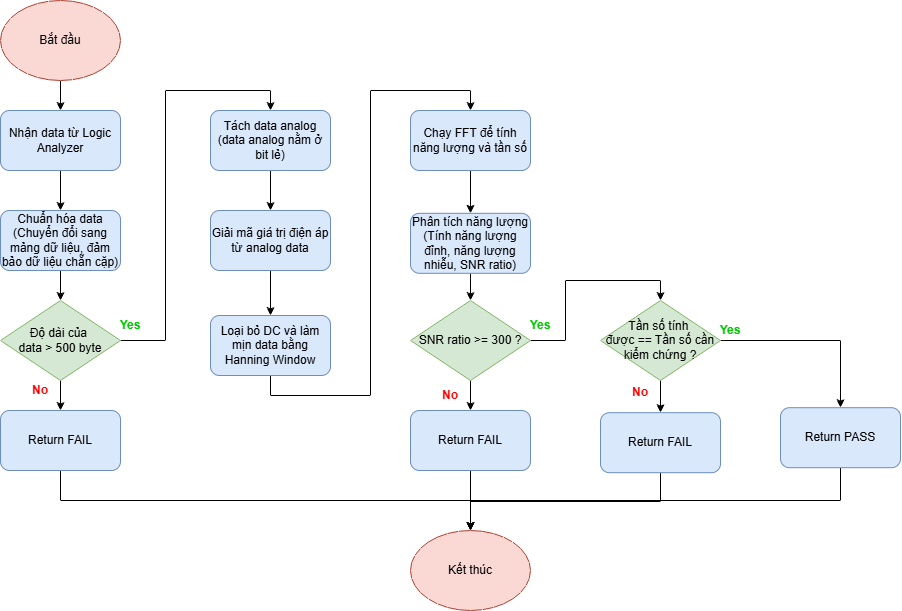
\includegraphics[width=0.8\textwidth]{image/verify_sine_wave_flowchart.png}
    \caption{Lưu đồ giải thuật xác minh sóng sine}
    \label{fig:verify_sine_wave_flowchart}
\end{figure}

Đối với bài kiểm tra sóng tam giác, dữ liệu tín hiệu sau khi xử lý FFT sẽ được phân tích theo đặc trưng phổ hài của sóng triangle. Cụ thể, hệ thống kiểm tra sự suy giảm của các harmonic bậc lẻ và mức năng lượng rất nhỏ của các harmonic bậc chẵn.

Nếu các harmonic chẵn đủ nhỏ và các harmonic lẻ giảm dần đúng đặc tính lý thuyết của sóng tam giác, hệ thống kết luận tín hiệu đầu ra đạt yêu cầu. Sau đó, tần số cơ bản của tín hiệu cũng được so sánh với giá trị mong đợi trong khoảng sai số cho phép.

Lưu đồ giải thuật chi tiết của quá trình xác minh sóng tam giác được trình bày trong Hình \ref{fig:verify_triangle_wave_flowchart}.

\begin{figure}[H]
    \centering
    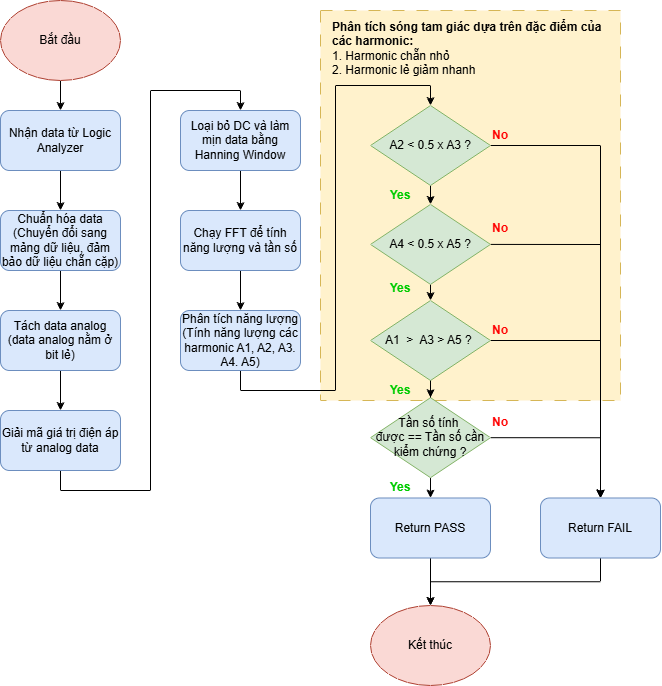
\includegraphics[width=0.8\textwidth]{image/verify_triangle_wave_flowchart.png}
    \caption{Lưu đồ giải thuật xác minh sóng tam giác}
    \label{fig:verify_triangle_wave_flowchart}
\end{figure}

\subsection{Kiểm tra ngoại vi PWM}

Mục đích của bài kiểm thử này là xác minh khả năng tạo tín hiệu điều chế độ rộng xung của DUT, đảm bảo firmware cấu hình đúng tần số và duty cycle của tín hiệu đầu ra theo yêu cầu thiết kế.

Trong bài kiểm thử này, DUT đóng vai trò chủ động phát sinh tín hiệu PWM tại chân đầu ra được chỉ định. Hệ thống Logic Analyzer được sử dụng để thu thập trực tiếp tín hiệu số tại chân PWM, sau đó dữ liệu được xử lý để xác định tần số thực tế và độ rộng xung nhằm so sánh với giá trị mong đợi.

Quy trình kiểm thử tổng quát bao gồm các bước sau:

\begin{itemize}
    \item Bước 1: Thiết lập môi trường kiểm thử bằng cách kết nối HIL, Logic Analyzer, cấp nguồn cho DUT và thiết lập kết nối với DUT.
    \item Bước 2: DUT được cấu hình tần số PWM mong muốn thông qua lệnh thiết lập tần số.
    \item Bước 3: DUT được cấu hình duty cycle tương ứng cho kênh PWM cần kiểm tra.
    \item Bước 4: DUT bắt đầu phát tín hiệu PWM tại chân đầu ra.
    \item Bước 5: Logic Analyzer thu thập dữ liệu tín hiệu số tại chân PWM trong khoảng thời gian xác định.
    \item Bước 6: Hệ thống thực hiện phân tích dữ liệu thu được để xác định tần số thực tế và duty cycle của tín hiệu PWM.
    \item Bước 7: So sánh kết quả đo với giá trị mong đợi trong khoảng sai số cho phép.
    \item Bước 8: DUT dừng phát tín hiệu PWM sau khi hoàn tất kiểm tra.
    \item Bước 9: Đánh giá kết quả kiểm thử và kết thúc môi trường kiểm thử.
\end{itemize}

Điều kiện đánh giá:

\begin{itemize}
    \item PASS: Tín hiệu PWM được tạo đúng với tần số và duty cycle mong đợi, sai số nằm trong giới hạn cho phép ($\pm 5\%$).
    \item FAIL: Tần số hoặc duty cycle đo được sai lệch vượt quá giới hạn cho phép, tín hiệu không được phát ra hoặc dữ liệu thu thập không đủ để phân tích.
\end{itemize}

Lưu đồ giải thuật tổng quát của bài kiểm thử được trình bày trong Hình \ref{fig:pwm_test_flowchart}.

\begin{figure}[H]
    \centering
    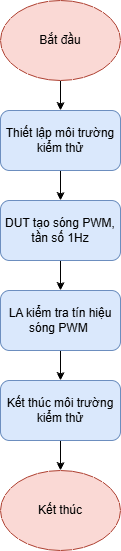
\includegraphics[height=0.4\textheight]{image/pwm_test_flowchart.png}
    \caption{Lưu đồ giải thuật tổng quát kiểm tra chức năng PWM}
    \label{fig:pwm_test_flowchart}
\end{figure}

Trong bài kiểm thử này, Logic Analyzer thực hiện thu thập dữ liệu số tại chân PWM và tách riêng kênh digital tương ứng để phân tích. Thuật toán kiểm tra được xây dựng dựa trên phương pháp phát hiện cạnh lên nhằm xác định chu kỳ tín hiệu.

Từ vị trí các cạnh lên liên tiếp, hệ thống tính toán thời gian của nhiều chu kỳ PWM để xác định tần số thực tế của tín hiệu. Đồng thời, tỷ lệ thời gian mức logic cao trên toàn bộ chu kỳ được sử dụng để tính duty cycle thực tế.

Sau khi thu được hai thông số này, hệ thống tiến hành so sánh với giá trị mong đợi đã cấu hình trước đó. Sai số cho phép được lựa chọn là $\pm 5\%$ nhằm phản ánh đúng đặc tính thực tế của hệ thống nhúng và giới hạn sai số đo của thiết bị.

Lưu đồ giải thuật chi tiết của quá trình xác minh tín hiệu PWM được trình bày trong Hình \ref{fig:verify_pwm_flowchart}.

\begin{figure}[H]
    \centering
    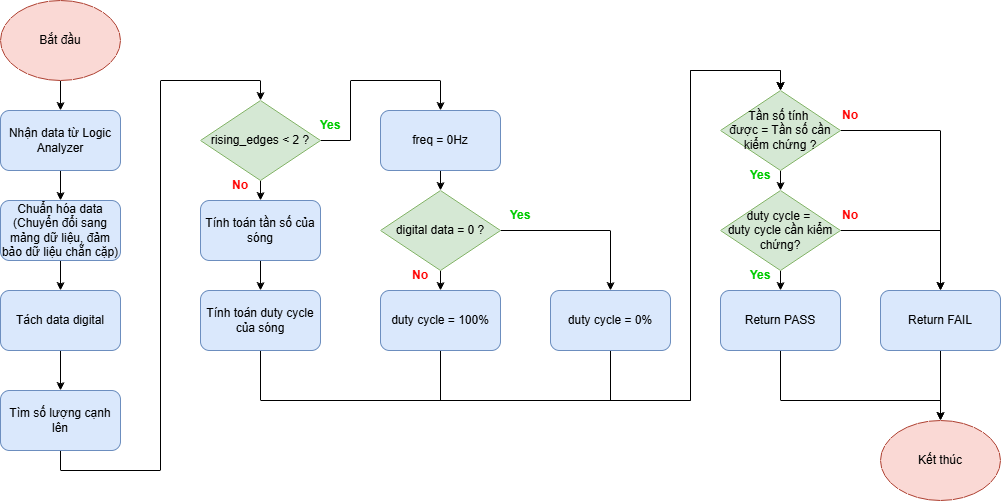
\includegraphics[width=0.85\textwidth]{image/verify_pwm_flowchart.png}
    \caption{Lưu đồ giải thuật xác minh tín hiệu PWM}
    \label{fig:verify_pwm_flowchart}
\end{figure}

\subsection{Kiểm tra ngoại vi UART}

Mục đích của bài kiểm thử này là xác minh khả năng truyền và nhận dữ liệu nối tiếp UART giữa DUT và hệ thống HIL, đảm bảo firmware cấu hình đúng giao tiếp UART và dữ liệu truyền nhận giữa hai thiết bị được thực hiện chính xác theo cả hai chiều.

Trong bài kiểm thử này, cả DUT và HIL đều được cấu hình giao tiếp UART với cùng thông số truyền thông như baudrate, số bit dữ liệu, bit chẵn lẻ và bit stop. Quá trình kiểm thử được thực hiện theo hai hướng truyền dữ liệu: từ DUT sang HIL và từ HIL sang DUT nhằm xác minh đầy đủ khả năng truyền nhận hai chiều của hệ thống.

Quy trình kiểm thử tổng quát bao gồm các bước sau:

\begin{itemize}
    \item Bước 1: Thiết lập môi trường kiểm thử bằng cách kết nối HIL, cấp nguồn cho DUT và thiết lập kết nối với DUT.
    \item Bước 2: Khởi tạo giao tiếp UART trên cả HIL và DUT với cùng cấu hình truyền thông.
    \item Bước 3: Thực hiện kiểm thử truyền dữ liệu từ DUT sang HIL bằng cách DUT gửi chuỗi dữ liệu kiểm thử và HIL đọc dữ liệu nhận được để so sánh với giá trị mong đợi.
    \item Bước 4: Thực hiện kiểm thử truyền dữ liệu từ HIL sang DUT bằng cách HIL gửi chuỗi dữ liệu kiểm thử và DUT đọc dữ liệu nhận được để so sánh với giá trị mong đợi.
    \item Bước 5: Đánh giá kết quả kiểm thử dựa trên toàn bộ phản hồi thu được từ cả hai chiều truyền dữ liệu.
    \item Bước 6: Kết thúc môi trường kiểm thử bằng cách ngắt kết nối DUT, tắt nguồn DUT và ngắt kết nối HIL.
\end{itemize}

Điều kiện đánh giá:

\begin{itemize}
    \item PASS: Dữ liệu truyền nhận ở cả hai chiều DUT → HIL và HIL → DUT đều chính xác, chuỗi nhận được khớp hoàn toàn với chuỗi dữ liệu mong đợi.
    \item FAIL: Có ít nhất một chiều truyền dữ liệu bị lỗi, dữ liệu nhận được không đầy đủ, sai nội dung hoặc không nhận được phản hồi.
\end{itemize}

Lưu đồ giải thuật tổng quát của bài kiểm thử được trình bày trong Hình \ref{fig:uart_test_flowchart}.

\begin{figure}[H]
    \centering
    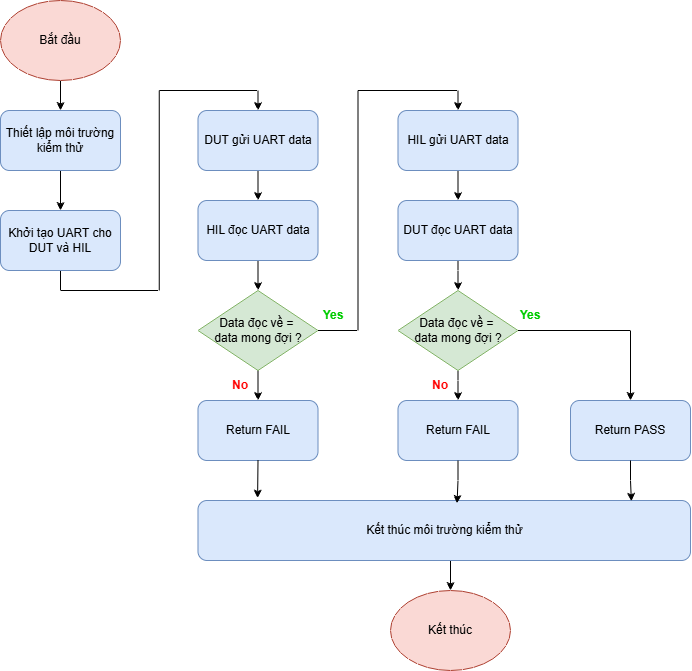
\includegraphics[width=0.8\textwidth]{image/uart_test_flowchart.png}
    \caption{Lưu đồ giải thuật tổng quát kiểm tra chức năng UART}
    \label{fig:uart_test_flowchart}
\end{figure}

\subsection{Kiểm tra ngoại vi CAN}

(Nên chia nhỏ bài test ra để test từng chức năng riêng: CAN receive, CAN transmit thay vì gộp chung như hiện tại. Cần Update thêm function cho CAN test case: Long Payload Transmission, Continuous Transmission)

Mục đích của bài kiểm thử này là xác minh khả năng truyền và nhận dữ liệu của DUT thông qua giao tiếp CAN, đảm bảo firmware cấu hình đúng ngoại vi CAN và dữ liệu trao đổi giữa DUT với hệ thống HIL được thực hiện chính xác, ổn định và không xảy ra lỗi truyền thông.

Trong bài kiểm thử này, hệ thống HIL đóng vai trò mô phỏng node giao tiếp CAN với DUT. HIL thực hiện gửi các khung dữ liệu CAN đến DUT, đồng thời đọc dữ liệu phản hồi từ DUT để kiểm tra tính chính xác của quá trình truyền nhận. Việc kiểm thử được thực hiện với cả dữ liệu dạng buffer tuần tự và dữ liệu dạng chuỗi ký tự nhằm đánh giá nhiều tình huống truyền thông khác nhau.

Quy trình kiểm thử tổng quát bao gồm các bước sau:

\begin{itemize}
    \item Bước 1: Thiết lập môi trường kiểm thử bằng cách kết nối HIL và cấp nguồn cho DUT.
    \item Bước 2: Hệ thống HIL gửi một khung dữ liệu CAN dạng buffer tuần tự đến DUT để kiểm tra khả năng truyền nhận dữ liệu nhị phân.
    \item Bước 3: HIL đọc dữ liệu phản hồi từ DUT và kiểm tra tính đúng đắn của dữ liệu bằng quy tắc tăng tuần tự giữa các byte.
    \item Bước 4: Hệ thống HIL gửi một chuỗi dữ liệu dạng ký tự đến DUT thông qua giao tiếp CAN để kiểm tra khả năng xử lý dữ liệu dạng text.
    \item Bước 5: HIL tiếp tục đọc dữ liệu phản hồi từ DUT và so sánh với chuỗi dữ liệu mong đợi.
    \item Bước 6: Đánh giá kết quả kiểm thử dựa trên toàn bộ phản hồi thu được.
    \item Bước 7: Kết thúc môi trường kiểm thử bằng cách ngắt kết nối HIL.
\end{itemize}

Điều kiện đánh giá:

\begin{itemize}
    \item PASS: Dữ liệu CAN nhận được từ DUT ở cả hai bài kiểm thử buffer và string đều chính xác, đúng thứ tự và khớp với giá trị mong đợi.
    \item FAIL: Có ít nhất một khung dữ liệu bị mất, sai nội dung, sai thứ tự hoặc DUT không phản hồi dữ liệu CAN đúng yêu cầu.
\end{itemize}

Lưu đồ giải thuật tổng quát của bài kiểm thử được trình bày trong Hình \ref{fig:can_test_flowchart}.

\begin{figure}[H]
    \centering
    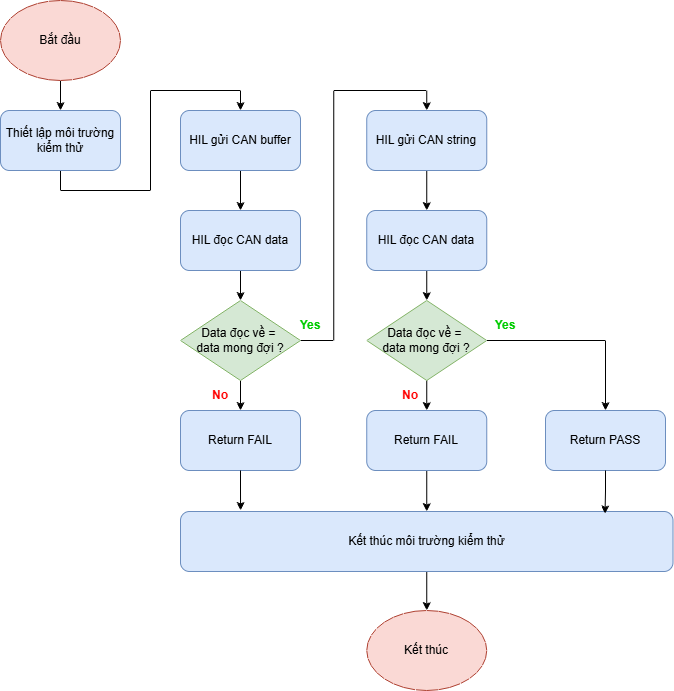
\includegraphics[width=0.8\textwidth]{image/can_test_flowchart.png}
    \caption{Lưu đồ giải thuật tổng quát kiểm tra chức năng CAN}
    \label{fig:can_test_flowchart}
\end{figure}

\subsection{Kiểm tra giao tiếp I2C với EEPROM}

Mục đích của bài kiểm thử này là xác minh khả năng giao tiếp giữa DUT và bộ nhớ ngoài EEPROM thông qua giao thức I2C, đảm bảo firmware cấu hình đúng ngoại vi I2C, thực hiện ghi và đọc dữ liệu chính xác, đồng thời đáp ứng yêu cầu về thời gian ghi dữ liệu.

Trong bài kiểm thử này, hệ thống HIL đóng vai trò mô phỏng thiết bị EEPROM với các tham số cấu hình như địa chỉ I2C, dung lượng bộ nhớ và kích thước trang. DUT thực hiện các thao tác đọc và ghi dữ liệu lên EEPROM thông qua giao tiếp I2C, sau đó phản hồi kết quả về PC để phục vụ quá trình đánh giá.

Quy trình kiểm thử tổng quát bao gồm các bước sau:

\begin{itemize}
    \item Bước 1: Thiết lập môi trường kiểm thử bằng cách kết nối HIL, cấp nguồn cho DUT và thiết lập kết nối với DUT.
    \item Bước 2: Hệ thống HIL khởi tạo mô hình EEPROM với các tham số cấu hình (địa chỉ, dung lượng, kích thước trang) và kích hoạt thiết bị trên bus I2C.
    \item Bước 3: DUT thực hiện khởi tạo giao tiếp với EEPROM thông qua I2C.
    \item Bước 4: DUT thực hiện ghi dữ liệu xuống EEPROM và đo thời gian ghi tương ứng với một khối dữ liệu xác định.
    \item Bước 5: Hệ thống kiểm thử đánh giá thời gian ghi có nằm trong giới hạn cho phép hay không.
    \item Bước 6: DUT thực hiện ghi và đọc lại dữ liệu từ EEPROM, sau đó gửi dữ liệu đọc được về PC.
    \item Bước 7: Hệ thống kiểm thử so sánh dữ liệu đọc được với dữ liệu mong đợi để xác minh tính toàn vẹn dữ liệu.
    \item Bước 8: Đánh giá kết quả kiểm thử dựa trên toàn bộ phản hồi thu được.
    \item Bước 9: Kết thúc môi trường kiểm thử bằng cách giải phóng tài nguyên EEPROM trên HIL.
\end{itemize}

\textbf{Điều kiện đánh giá:}

\begin{itemize}
    \item PASS: 
    \begin{itemize}
        \item HIL khởi tạo EEPROM thành công.
        \item DUT truy cập được EEPROM tại địa chỉ đã cấu hình.
        \item Thời gian ghi dữ liệu của DUT nhỏ hơn ngưỡng cho phép.
        \item Dữ liệu ghi vào EEPROM được đọc lại chính xác, đúng thứ tự và không bị sai lệch.
    \end{itemize}

    \item FAIL: Bài kiểm thử sẽ trả về FAIL nếu xảy ra bất kỳ lỗi nào sau đây:
    \begin{itemize}
        \item HIL không khởi tạo được EEPROM (sai địa chỉ, sai giá trị cấu hình).
        \item EEPROM không được phát hiện trên bus I2C.
        \item DUT không giao tiếp được với EEPROM (không phát hiện được thiết bị hoặc không đọc/ghi được).
        \item Thời gian ghi dữ liệu vượt quá ngưỡng cho phép.
        \item Dữ liệu đọc lại không khớp với dữ liệu đã ghi (mất dữ liệu, sai thứ tự).
    \end{itemize}
\end{itemize}

Lưu đồ giải thuật tổng quát của bài kiểm thử được trình bày trong Hình \ref{fig:eeprom_test_flowchart}.

\begin{figure}[H]
    \centering
    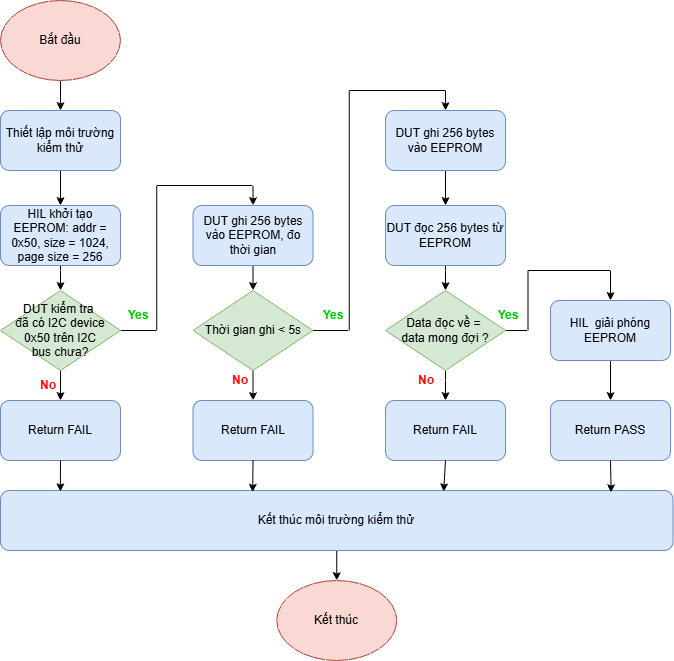
\includegraphics[width=0.8\textwidth]{image/eeprom_test_flowchart.png}
    \caption{Lưu đồ giải thuật kiểm tra chức năng EEPROM thông qua giao tiếp I2C}
    \label{fig:eeprom_test_flowchart}
\end{figure}.

\subsection{Kiểm tra giao tiếp I2C với RTC}

Mục đích của bài kiểm thử này là xác minh khả năng giao tiếp giữa DUT với bộ thời gian thực RTC.

Trong bài kiểm thử này, hệ thống HIL đóng vai trò mô phỏng và kích hoạt thiết bị RTC trên bus I2C. DUT thực hiện các thao tác thiết lập và đọc dữ liệu từ RTC, sau đó gửi kết quả về PC để phục vụ quá trình kiểm tra và đánh giá.

Quy trình kiểm thử tổng quát bao gồm các bước sau:

\begin{itemize}
    \item Bước 1: Thiết lập môi trường kiểm thử bằng cách kết nối HIL, cấp nguồn cho DUT và thiết lập kết nối với DUT.
    \item Bước 2: HIL khởi tạo thiết bị RTC tại địa chỉ I2C tương ứng và kích hoạt thiết bị trên bus.
    \item Bước 3: DUT khởi tạo RTC và thiết lập thời gian (giờ, phút, giây) và ngày tháng (thứ, ngày, tháng, năm).
    \item Bước 4: DUT đọc lại giá trị thời gian và ngày tháng từ RTC, hệ thống so sánh với giá trị mong đợi trong khoảng sai số cho phép.
    \item Bước 5: Kiểm tra khả năng tự động tăng thời gian của RTC bằng cách thiết lập thời điểm gần thời điểm chuyển ngày, sau đó chờ một khoảng thời gian xác định.
    \item Bước 6: DUT đọc lại thời gian và ngày tháng sau khi chờ, hệ thống kiểm tra việc chuyển sang ngày mới và giá trị thời gian có đúng hay không.
    \item Bước 7: Đánh giá kết quả kiểm thử dựa trên toàn bộ dữ liệu thu được.
    \item Bước 8: Kết thúc môi trường kiểm thử bằng cách tắt nguồn DUT và ngắt kết nối HIL.
\end{itemize}

\textbf{Điều kiện đánh giá:}

\begin{itemize}
    \item PASS:
    \begin{itemize}
        \item HIL khởi tạo và kích hoạt thành công thiết bị RTC trên bus I2C.
        \item DUT thiết lập và đọc lại chính xác giá trị thời gian và ngày tháng từ RTC.
        \item Sai số thời gian nằm trong khoảng cho phép (do độ trễ xử lý và thời gian giao tiếp).
        \item RTC tự động tăng thời gian chính xác và chuyển ngày đúng khi vượt qua mốc 00:00:00.
    \end{itemize}

    \item FAIL: Bài kiểm thử sẽ trả về FAIL nếu xảy ra bất kỳ lỗi nào sau đây:
    \begin{itemize}
        \item HIL không khởi tạo hoặc không kích hoạt được thiết bị RTC.
        \item DUT không giao tiếp được với RTC (không đọc/ghi được dữ liệu).
        \item Giá trị thời gian hoặc ngày tháng đọc được không khớp với giá trị đã thiết lập.
        \item Sai số thời gian vượt quá ngưỡng cho phép.
        \item RTC không tăng thời gian đúng hoặc không chuyển ngày khi vượt qua mốc thời gian.
    \end{itemize}
\end{itemize}

Lưu đồ giải thuật tổng quát của bài kiểm thử được trình bày trong Hình \ref{fig:rtc_test_flowchart}.

\begin{figure}[H]
    \centering
    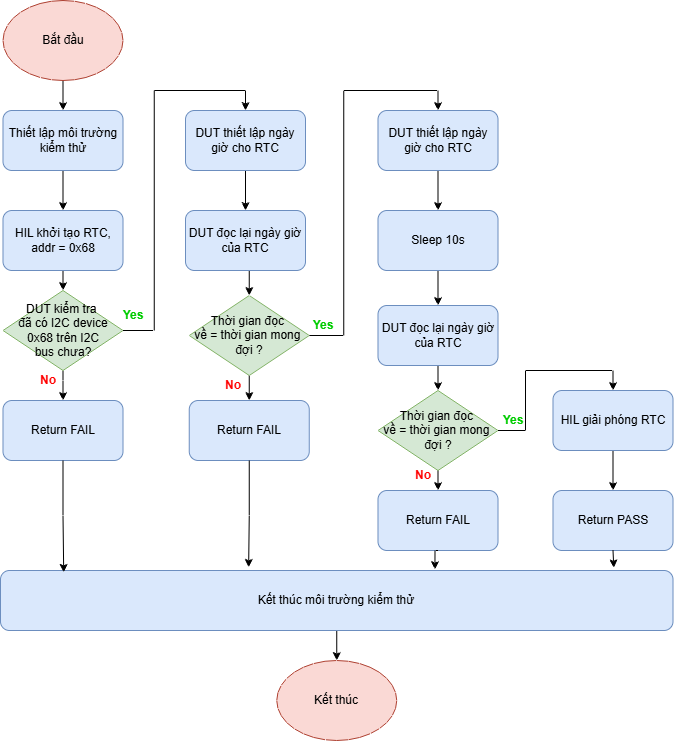
\includegraphics[width=0.8\textwidth]{image/rtc_test_flowchart.png}
    \caption{Lưu đồ giải thuật tổng quát kiểm tra chức năng RTC}
    \label{fig:rtc_test_flowchart}
\end{figure}

\subsection{Kiểm tra giao tiếp SPI với FLASH}

Mục đích của bài kiểm thử này là xác minh khả năng giao tiếp và thao tác với bộ nhớ SPI Flash của DUT, bao gồm việc đọc ID thiết bị, đọc dữ liệu, ghi dữ liệu và xóa dữ liệu. Bài kiểm thử nhằm đảm bảo firmware cấu hình đúng giao tiếp SPI và các thao tác trên bộ nhớ Flash được thực hiện chính xác, ổn định.

Trong bài kiểm thử này, hệ thống HIL đóng vai trò chuẩn bị dữ liệu mẫu trong SPI Flash để DUT đọc và kiểm tra. DUT thực hiện các thao tác đọc, ghi và xóa dữ liệu trên SPI Flash, sau đó gửi kết quả về PC để tiến hành đánh giá.

Quy trình kiểm thử tổng quát bao gồm các bước sau:

\begin{itemize}
    \item Bước 1: Thiết lập môi trường kiểm thử bằng cách kết nối HIL, cấp nguồn cho DUT và thiết lập kết nối với DUT.
    \item Bước 2: DUT thực hiện đọc ID của SPI Flash để xác minh kết nối phần cứng và nhận diện thiết bị.
    \item Bước 3: HIL chuẩn bị dữ liệu mẫu với độ dài xác định (512 bytes) trong bộ nhớ SPI Flash.
    \item Bước 4: DUT đọc dữ liệu từ SPI Flash và hệ thống kiểm tra tính đúng đắn của dữ liệu theo quy luật tăng tuần tự.
    \item Bước 5: DUT thực hiện xóa dữ liệu trong SPI Flash.
    \item Bước 6: DUT đọc lại dữ liệu sau khi xóa và hệ thống kiểm tra trạng thái dữ liệu đã được xóa hoàn toàn.
    \item Bước 7: DUT ghi dữ liệu mới vào SPI Flash với độ dài lớn hơn (1024 bytes).
    \item Bước 8: DUT đọc lại dữ liệu vừa ghi và hệ thống kiểm tra tính chính xác của dữ liệu.
    \item Bước 9: Đánh giá kết quả kiểm thử dựa trên toàn bộ dữ liệu thu được.
    \item Bước 10: Kết thúc môi trường kiểm thử bằng cách ngắt kết nối HIL và DUT.
\end{itemize}

\textbf{Điều kiện đánh giá:}

\begin{itemize}
    \item PASS:
    \begin{itemize}
        \item DUT đọc được đúng ID của SPI Flash, xác nhận thiết bị hoạt động bình thường.
        \item Dữ liệu đọc từ SPI Flash (do HIL chuẩn bị) chính xác và đúng thứ tự.
        \item Sau khi thực hiện lệnh xóa, toàn bộ dữ liệu trong vùng nhớ được đưa về trạng thái đã xóa (thường là 0xFF).
        \item Dữ liệu ghi mới vào SPI Flash được đọc lại chính xác, không bị sai lệch.
    \end{itemize}

    \item FAIL: Bài kiểm thử sẽ trả về FAIL nếu xảy ra bất kỳ lỗi nào sau đây:
    \begin{itemize}
        \item DUT không đọc được ID hoặc ID không đúng với thiết bị SPI Flash.
        \item Dữ liệu đọc từ SPI Flash bị sai, thiếu hoặc không đúng thứ tự.
        \item Quá trình xóa không thành công (dữ liệu sau khi xóa không đồng nhất).
        \item Dữ liệu ghi vào SPI Flash bị sai lệch khi đọc lại.
        \item DUT không phản hồi hoặc xảy ra lỗi trong quá trình giao tiếp SPI.
    \end{itemize}
\end{itemize}

Lưu đồ giải thuật tổng quát của bài kiểm thử được trình bày trong Hình \ref{fig:spi_flash_test_flowchart}.

\begin{figure}[H]
    \centering
    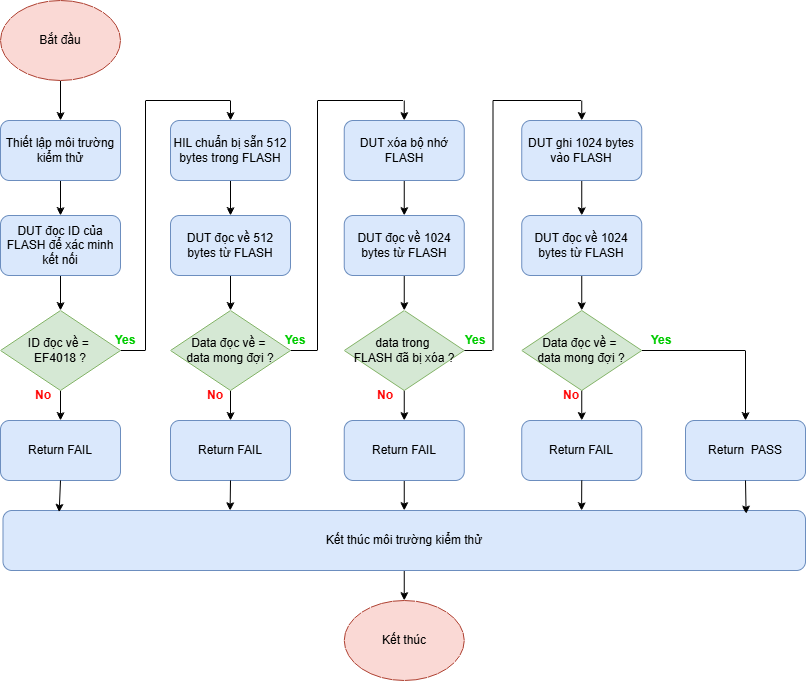
\includegraphics[width=0.8\textwidth]{image/spi_flash_test_flowchart.png}
    \caption{Lưu đồ giải thuật tổng quát kiểm tra chức năng SPI Flash}
    \label{fig:spi_flash_test_flowchart}
\end{figure}
.